\documentclass[aspectratio=169,10pt]{beamer}
\usetheme{metropolis}
\usepackage{amsmath,amssymb}
\usepackage{graphicx}
\definecolor{acc}{HTML}{00798C}
\setbeamercolor{alerted text}{fg=acc}
\newcommand{\Lik}{\mathcal{L}}
\title{Bayesian spectral deconvolution with Hamiltonian Monte Carlo}
\subtitle{How many peaks are in my spectrum --- and where?}
\author{Jeroen Sangers}
\date{Group meeting, \today}
\begin{document}
\maketitle

% ---------------------------------------------------------------
\begin{frame}{1. The problem: blurred, noisy spectra}
\small
\begin{columns}[T]
\begin{column}{0.58\textwidth}
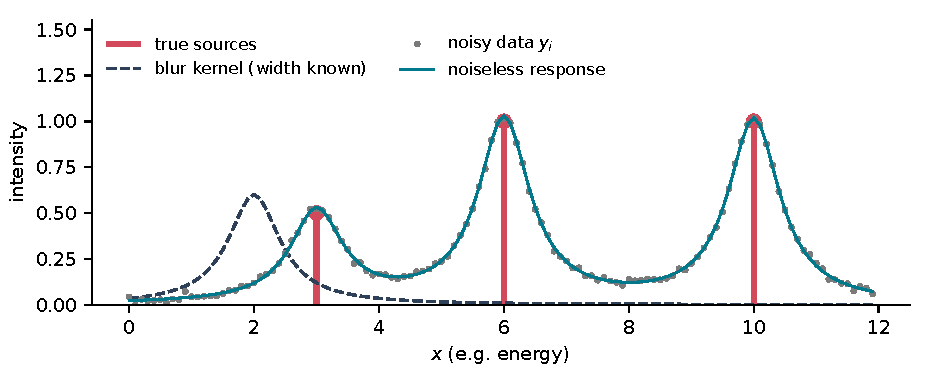
\includegraphics[width=\linewidth]{figs/fig1_problem.pdf}
\end{column}
\begin{column}{0.4\textwidth}
Measured spectrum = sum of $K$ blurred sources + noise:
\[
y_i=\sum_{k=1}^{K} I_k\,\phi(x_i-\mu_k)+\varepsilon_i,\qquad \varepsilon_i\sim\mathcal N(0,\sigma^2)
\]
with a Lorentzian kernel of known width $\gamma$:
\[
\phi(x-\mu)=\frac{1}{1+\big((x-\mu)/\gamma\big)^{2}}
\]
\vspace{2pt}
Unknowns: $\boldsymbol\theta=(I_1..I_K,\mu_1..\mu_K)$ \\[3pt]
\alert{Two questions:} what are $\boldsymbol\theta$, and \alert{what is $K$?}
\end{column}
\end{columns}
\end{frame}

% ---------------------------------------------------------------
\begin{frame}{2. Bayes: a distribution over parameters, not a single fit}
\[
p(\boldsymbol\theta\,|\,y,K)=\frac{p(y\,|\,\boldsymbol\theta,K)\;p(\boldsymbol\theta\,|\,K)}{Z_K},
\qquad Z_K=\int \Lik(\boldsymbol\theta)\,p(\boldsymbol\theta)\,d\boldsymbol\theta
\]
\centering {\small posterior $=$ likelihood $\times$ prior $/$ evidence}\par\medskip\raggedright
\begin{columns}[T]
\begin{column}{0.5\textwidth}
\textbf{Likelihood} (Gaussian noise)
\[
\log\Lik=-\frac{1}{2\sigma^2}\sum_i\Big(y_i-\sum_k I_k\phi(x_i-\mu_k)\Big)^2+\text{const}
\]
\textbf{Priors} (uniform boxes)
\[
I_k\sim U(0.2,1.2),\qquad \mu_k\sim U(1,11)
\]
\end{column}
\begin{column}{0.46\textwidth}
\textbf{Why sample?}
\begin{itemize}
\item Posterior of $\boldsymbol\theta$ is non-Gaussian and multimodal
\item We want error bars, not just a best fit
\item $Z_K$ needs an integral over $2K$ dimensions
\end{itemize}
\vspace{4pt}
$\Rightarrow$ Markov chain Monte Carlo: draw samples $\boldsymbol\theta^{(s)}\sim p(\boldsymbol\theta|y,K)$
\end{column}
\end{columns}
\end{frame}

% ---------------------------------------------------------------
\begin{frame}{3. Hamiltonian Monte Carlo: let the posterior push the sampler}
\small
\begin{columns}[T]
\begin{column}{0.46\textwidth}
Treat $\boldsymbol\theta$ as a position in potential $U$, add a fictitious momentum $\mathbf p$:
\[
U(\boldsymbol\theta)=-\log\Lik-\log p(\boldsymbol\theta),\quad
H=U(\boldsymbol\theta)+\tfrac12\mathbf p^{\top}\mathbf p
\]
Leapfrog steps (step size $\epsilon$):
\begin{align*}
\mathbf p&\leftarrow \mathbf p-\tfrac{\epsilon}{2}\nabla U,\\
\boldsymbol\theta&\leftarrow \boldsymbol\theta+\epsilon\,\mathbf p,\\
\mathbf p&\leftarrow \mathbf p-\tfrac{\epsilon}{2}\nabla U
\end{align*}
Accept with $\min\!\big(1,e^{-\Delta H}\big)$.
\vspace{3pt}

\alert{Long, informed moves} instead of random-walk steps; the gradient $\nabla U$ points where the fit improves.
\end{column}
\begin{column}{0.52\textwidth}
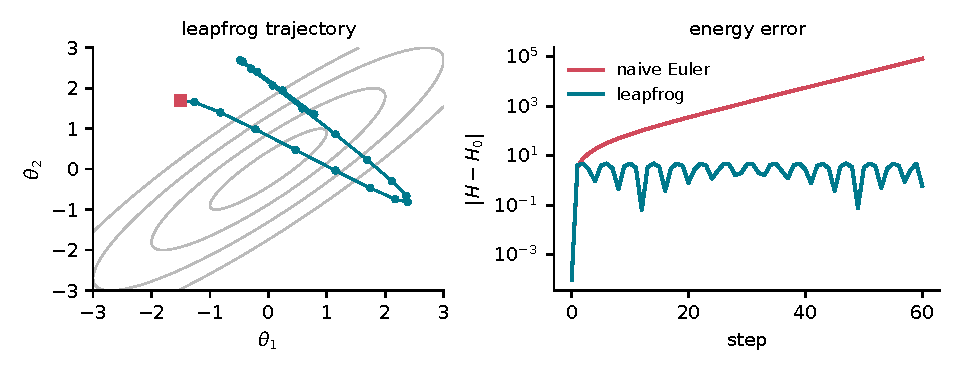
\includegraphics[width=\linewidth]{figs/fig3_hmc.pdf}

{\footnotesize Toy 2D correlated Gaussian. Leapfrog nearly conserves $H$, so proposals far away are still accepted (notebook: $\approx 80\%$ at $\beta=1$).}
\end{column}
\end{columns}
\end{frame}

% ---------------------------------------------------------------
\begin{frame}{4. Parallel tempering: escaping local optima}
\small
\begin{columns}[T]
\begin{column}{0.47\textwidth}
Run chains at inverse temperatures $0\le\beta_1<\dots<\beta_L=1$:
\[
p_\beta(\boldsymbol\theta\,|\,y)\;\propto\;\Lik(\boldsymbol\theta)^{\beta}\,p(\boldsymbol\theta)
\]
\begin{itemize}
\item $\beta=0$: prior (explores everything)
\item $\beta=1$: true posterior (the answer)
\end{itemize}
Neighbouring chains swap states with probability
\[
\min\!\Big\{1,\;e^{(\beta_i-\beta_j)(E_i-E_j)}\Big\},\quad E=-\log\Lik
\]
Hot chains find new modes; swaps hand them to the cold chain.

{\scriptsize Notebook: 36 temperatures, HMC in each chain, swap every 10 steps, mean swap acceptance $\approx 0.6$--$0.7$.}
\end{column}
\begin{column}{0.51\textwidth}
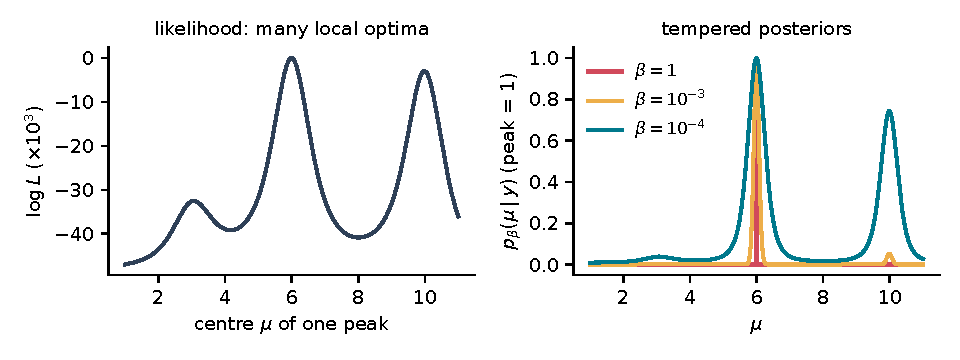
\includegraphics[width=\linewidth]{figs/fig4_tempering.pdf}

{\footnotesize Profile of the likelihood over one peak position for our data: several optima at $\beta=1$, a nearly flat landscape at small $\beta$.}
\end{column}
\end{columns}
\end{frame}

% ---------------------------------------------------------------
\begin{frame}{5. Choosing $K$: the evidence from the temperature ladder}
\begin{columns}[T]
\begin{column}{0.55\textwidth}
Tempering also gives $Z_K$ for free. With $Z(\beta)=\int \Lik^{\beta}p\,d\boldsymbol\theta$, $Z(0)=1$:
\[
\log Z_K=\sum_{l=1}^{L-1}\log\frac{Z(\beta_{l+1})}{Z(\beta_l)},\qquad
\frac{Z(\beta_{l+1})}{Z(\beta_l)}=\Big\langle \Lik^{\,\beta_{l+1}-\beta_l}\Big\rangle_{\beta_l}
\]
each term is a plain average over samples of chain $l$.\\[6pt]
\textbf{Stochastic complexity} $F(K)=-\log Z_K$; choose $K^\ast=\arg\min_K F(K)$.

\vspace{4pt}
\alert{Automatic Occam's razor:} extra peaks fit slightly better but spread the prior over more volume, so $Z_K$ drops.
\end{column}
\begin{column}{0.42\textwidth}
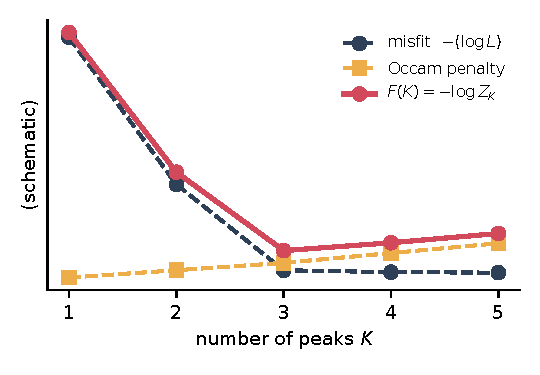
\includegraphics[width=\linewidth]{figs/fig5_evidence.pdf}

{\footnotesize Schematic of the trade-off. Least-squares $\chi^2$ on our data: $K{=}2$: 19\,700, $K{=}3$: 138 (120 points), $K{=}4$: 137.}
\end{column}
\end{columns}
\end{frame}

% ---------------------------------------------------------------
\begin{frame}{6. Result on the synthetic spectrum}
\small
\begin{columns}[T]
\begin{column}{0.6\textwidth}
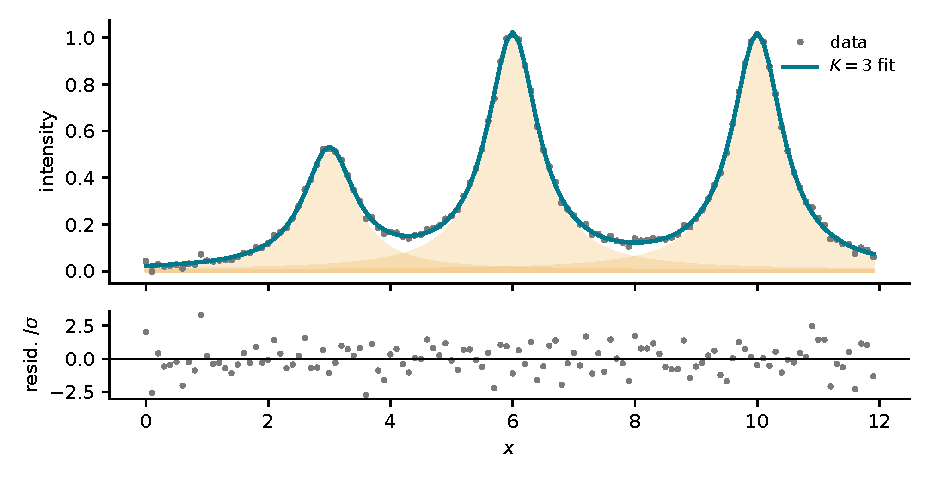
\includegraphics[width=\linewidth]{figs/fig6_result.pdf}
\end{column}
\begin{column}{0.37\textwidth}
Three true peaks at $\mu=3,6,10$; evidence compared for $K=2,3,4$.

\alert{$K^\ast=3$} selected. Posterior (cold chain):
\begin{center}
\small
\begin{tabular}{ccc}
$\mu_k$ & $\pm$ & $I_k$\\\hline
3.004 & 0.003 & 0.49\\
6.001 & 0.002 & 1.00\\
10.001 & 0.002 & 0.99
\end{tabular}
\end{center}
\textbf{Take-aways}
\begin{itemize}
\item HMC: efficient moves in $2K$ dims
\item Tempering: no local traps, gives $Z_K$
\item $K$ chosen without heuristics
\end{itemize}
\end{column}
\end{columns}
\end{frame}
\end{document}
